\section{Implementation}

\subsection{Defined Primitives and \texttt{main()}}
    The first step taken in beginning the actual implementation was to define a collection of primitive types. This was done for a number of reasons. Firstly, the typical built-in types provided in C++ (e.g. \texttt{unsigned int}) have a size that is dependent on the target system and compiler used. The standard library header \texttt{cstdint} provides types such as \texttt{uint16\_t} which are of a definite size (unsigned 16-bit integer in the case of the aforementioned).

    \inputminted{c++}{code/primitives.hpp}

    Testing and review are not really applicable at this early stage of development.

\subsection{Headers for \texttt{Memory} and \texttt{Intel8086} Classes}
    An element of the C++ compilation system is that it is advantageous in terms of compile time to keep the declaration of class separate from the implementation of any of its member functions. Class declarations are defined in header files (\texttt{.cpp}) while class implementations are defined in source files (\texttt{.hpp}). At this early stage is development, I find it beneficial to create headers to give an overall structure of classes before beginning their actual implementation.

    As such, a header for the \texttt{Intel8086} class was created at this stage in development. As for the \texttt{Memory} class, due to it actually being a class template (meaning implementation cannot be put into a separate \texttt{.cpp} file) and also fairly simplistic, it was declared and implemented during this stage of development in the header file shown below.

    \inputminted{c++}{code/memory.hpp}

    \inputminted{c++}{code/intel8086.hpp}

    \subsubsection{Testing}
        As the \texttt{Memory} class was actually implemented fully at this stage due to the aforementioned reasons, writing unit tests to ensure it functions as expected is now possible. This is not the case for \texttt{Intel8086} class so that will be tested later in development once it is fully implemented.

        \inputminted{c++}{code/testmemory.cpp}

        \begin{figure}[h]
            \centering
            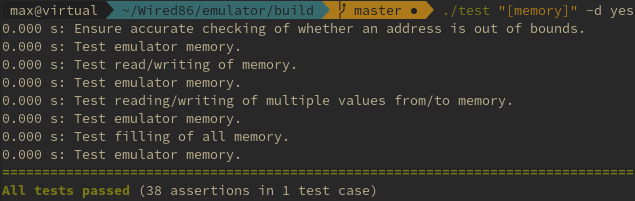
\includegraphics[scale=0.6]{memory-tests}
            \caption{Results of memory unit tests (all tests passed).}
            \label{fig:memory-tests}
        \end{figure}

        See figure \ref{fig:memory-tests} for the results of the aforementioned unit tests.

    \subsubsection{Review}
        You will notice that the \texttt{Memory::OutOfBounds} exception class is defined as a subclass of \texttt{std::exception}. After some research, it has come to my attention that it would be more beneficial to define it as a subclass of \texttt{std::runtime\_error} instead as this allows the specification of an error message to be returned by the inherited \texttt{what()} method. This is something I will address in a subsequent stage of development.

        In addition, there exists a 'to do' comment in the emulator memory header specifying that functions for reading and writing emulator memory from/to a file still need to be provided. Again, this something I will address later in development.

        As for the CPU header, I am currently satisfied with the general manner with which the class will operate. The address of instruction pointer segmented within the code segment is returned by the \texttt{nextInstructionAddress} method. This address and a memory object can then be passed to the \texttt{fetchDecodeInstruction} method which will return an appropriate object that inherits from \texttt{Instruction} (enclosed within a \texttt{std::unique\_ptr}). This \texttt{Instruction}-derived object can then passed to \texttt{executeInstruction} where it is actually run. This provides a fair degree of flexibility - the separation of decoding and executing gives the freedom to decode an instruction at a given address (so that its assembly representation may be seen, for example) without then being forced to execute it.

\subsection{CPU Registers}
    Registers are represented using a separate class to that of the CPU itself. Internally, I decided to use a class template system so that an enumeration type can be used as a register index. This has several benefits over other potential methods of implementing registers. For example, other projects that I have researched simply accepted integers as indexes to an array representing CPU registers. This is problematic as any integer constant can be used, even a totally unrelated constant or out-of-bound value. By using a type-specific enumeration, only appropriate register indexes can be passed without causing a type-error.

    \inputminted{c++}{code/registerindexes.hpp}

    You'll notice that the register indexes are not actually C++ enumerations defined with the \texttt{enum} keyword. Rather, they are classes emulating enumerations in style similar to that of Java's enumerations. This is beneficial as it allows register indexes to have additional properties (for example, a string description of its purpose).

    \inputminted{c++}{code/registers.hpp}

    Naturally, a lot of the code is not implemented at this stage.

\subsection{\texttt{conversion} Namespace}
    Something I felt would be useful to do after working on register indexes, was to provide a collection of helper/conversion functions under a \texttt{conversion} namespace. 

    \inputminted{c++}{code/conversion.hpp}

    \inputminted{c++}{code/conversion.cpp}

    This allows me to improve code readability by replacing code such as: \mint[linenos=false]{c++}{return get(index) & 0xFF;} seen in the \texttt{RegistersLowHigh} class with: \mint[linenos=false]{c++}{return conversion::getHighByte(get(index));}

\subsection{Logging}
    Before a functional GUI is implemented, I will have to rely on a command-line interface for input and output. As such, building a proper system for clear, organised output seemed vital. Before writing the code for this logging system, I decided on several key features that said system would need to have:
    \begin{itemize}
        \item Provide different output types (information, success, warning, error).
        \item Colour-code output types.
        \item Include timestamps for each logged message.
    \end{itemize}

    \inputminted{c++}{code/logging.hpp}

    \inputminted{C++}{code/logging.cpp}

\subsection{Build Script}
    It was at this point that the first proper build system was set up. Up until this point, I had been manually running a series of commands to build the project as necessary. As mentioned earlier in this document, I plan to use the CMake build system which (on my Linux system) relies on GCC Make and G++ compiler. See below for the \texttt{CMakeLists.txt} file.

    \inputminted{cmake}{code/CMakeLists.txt}

    \subsubsection{Testing}
        The build script is so simple at this stage that there isn't much to test beyond ensuring it actually compiles the program successfully.

    \subsubsection{Review}
        This script will later be improved upon to allow for multiple build types.

\subsection{Added Registers to CPU}
    With CPU register representation implemented (see section \ref{}), it is now possible to add these registers as members of the CPU class.

    \inputminted[linenos=false]{c++}{code/intel8086_registers.hpp}

\subsection{Memory Exception}
    One of the features of C++ over C is the concept of exceptions. As you can see in the revised header file below, I made use of this feature by having an \texttt{OutOfBounds} exception class (derived from \texttt{std::runtime\_error}) nested within the \texttt{Memory} class template. This use of nested classes is beneficial as it means that a unique \texttt{OutOfBounds} class is created for each unique version of \texttt{Memory} template. This means that the exception class can make use of the template parameters of the memory class.

    In addition, I have also now implemented the read and writing of memory to and from files. This is something of a key feature as it allows the user to prepare programs to run on the emulator in advance and then load them to/from the software as need be.

    \inputminted{c++}{code/memory_bruh.hpp}

\subsection{}
